\section{Cinemática} \label{sec:cinematica}

La cinemática es una rama de la física que estudia el movimiento de los objetos sólidos en función del tiempo, sin considerar las causas (fuerzas) que lo originan. Este análisis se basa en variables como la posición, la velocidad y la aceleración, y considera tres elementos fundamentales: el espacio, el tiempo y el móvil. En el contexto de la robótica, se aplica especialmente a sistemas de cuerpos rígidos como los manipuladores, describiendo sus trayectorias sin involucrar dinámicas.

En robótica, la cinemática se clasifica principalmente en dos tipos: \textbf{cinemática directa} y \textbf{cinemática inversa}. La primera permite determinar la posición y orientación del efector final a partir de los valores articulares del robot, mientras que la segunda se enfoca en calcular los valores articulares que permiten alcanzar una posición y orientación deseadas del efector final.

\subsection{Cinemática Directa}

La cinemática directa (o directa geométrica) establece la relación entre los ángulos articulares del robot y la posición y orientación del efector final. Para esta tarea, comúnmente se emplea el método de Denavit-Hartenberg (DH), que permite representar de forma sistemática la configuración espacial del robot mediante transformaciones homogéneas.

Dichas transformaciones permiten obtener no solo la ubicación del efector final, sino también su orientación en el espacio. Además, conceptos como el jacobiano geométrico son fundamentales para analizar la velocidad y aceleración del sistema en función de sus variables articulares.

Un desarrollo detallado del análisis computacional aplicado a este modelo puede encontrarse en la \hyperref[sec:proceso_cinematica]{sección del proceso de Cinemática}.

\subsection{Cinemática Diferencial}

Dentro de la robótica la cinemática diferencial se enfoca en el estudio de cómo cambian las velocidades del robot conforme se van moviendo sus articulaciones. Se relacionan las velocidades articulares con las velocidades lineales y angulares del efector final. Nos permite calcular cómo se mueve y controlar la velocidad del efector final. 
El Jacobiano es una matriz la cual relaciona directamente estas dos velocidades. Está traduce velocidades del espacio articular al espacio cartesiano. El Jacobiano de un robot con n articulaciones tiene las siguientes características:
  \\
-6 filas \\
-n número de columnas.\\

\begin{figure}[h]
	\centering
	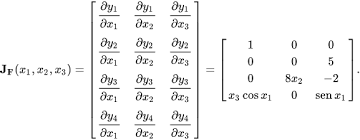
\includegraphics[width=0.5\linewidth]{img/jacobiano}
	\caption{Matriz de Jacobiano}
	\label{fig:jacobiano}
\end{figure}

\subsection{Cinemática Inversa}

La cinemática inversa es una rama de la robótica que se encarga de determinar los valores articulares que debe tener un robot para que su efector final alcance una posición y orientación específicas en el espacio. A diferencia de la cinemática directa, donde se conoce la configuración de las articulaciones y se calcula la posición del efector, en la cinemática inversa el objetivo es obtener la configuración articular a partir de una posición deseada.

El problema de la cinemática inversa suele ser más complejo que el de la cinemática directa, ya que no siempre existe una única solución. De hecho, puede haber múltiples soluciones, una sola solución o incluso ninguna, dependiendo de la estructura del robot y de la posición deseada.

Este análisis es esencial para tareas de planificación de movimientos y control, ya que permite determinar cómo deben moverse las articulaciones para que el robot realice acciones como tomar un objeto, seguir una trayectoria o posicionar una herramienta con precisión.

Existen diferentes métodos para resolver la cinemática inversa, incluyendo enfoques analíticos y numéricos. Los métodos analíticos se basan en álgebra y trigonometría, y son útiles cuando el robot tiene una estructura relativamente sencilla. Los métodos numéricos, como el descenso del gradiente o el uso del Jacobiano, son más versátiles y se utilizan cuando el sistema es complejo o no tiene una solución cerrada.
